\section{Certificates}
There are several techniques that have been proposed for the distribution of public keys. Virtually all these proposals can be grouped into the four general schemes
\begin{itemize}
    \item \textbf{Public announcement}: low overhead, no infrastructure required, but no trust (anyone can announce anything)
    \item \textbf{Public Directory}: there is a trusted entity to manage central service, but it needs to be online all the time, it fails if records get compromised and the registration requires an identity check
    \item \textbf{Public Key Authority}: it automates key exchange process and provides freshness through timestamps, but has the same problems of public directory
    \item \textbf{Public Key Certificates}: distribution does not require central authority
\end{itemize}

\paragraph{Definition} A certificate is a digitally-signed statement that binds a public key to some identifying information. The signer of the certificate is called its \textit{issuer} and the entity talked about in the certificate is the \textit{subject} of the certificate.\\

\noindent In order to believe to a certificates, we need to trust the issuer/signer not to lie to use and we also need to believe that it is hard to forge the digital signature on a signed document
\subsection{Strategies for CA Hierarchies}
Generally,in order to obtain a certificate
\begin{itemize}
    \item A user has to ask a \textit{Certification Authority} (CA) that issues certificates and asks for one
    \item The CA verifies the claim the user is making
    \item CA then issues the user a certificate for his public key
\end{itemize}
There are different viable hierarchies model to do so
\subsubsection{Monopoly}
Choose a universally trusted organization, embed their public key in everything and give them universal monopoly to issue certificates, so that everyone get certificates from them. There are several problems with this model:
\begin{itemize}
    \item If no one else is allowed to create certs, there is no incentive to offer competitive prices
    \item Getting certificates for remote user will be insecure or expensive
    \item The security of the world depends on the honesty and competence of that one organization, forever
\end{itemize}
\paragraph{Variation} Adding \textit{Registration Authorities} (RAs) that are trusted by the CA, so everyone can ask certificates to RAs, who in turn will ask to CA. In this way we solve the distance problem, but not the other issues.
\subsubsection{Oligarchy}
Have multiple trusted CAs. 
\paragraph{Variation} Allow trusted CAs to issue certificates for other CAs to the list of trusted CAs. This is similar to the monopoly variation, but is less efficient (end user must verify multiple certificates), faster (less delay for RA to get certificate) and less secure (multiple CA means multiple keys to trust).

\subsubsection{Anarchy}
Anyone signs certificates for anyone else. It is similar to Oligarchy variation, but user must consciously configure starting certificates. The problems are that it is hard to scale (computationally difficult to find path), it is not practical to decide if certain path should be trusted (too many decisions for the end user).

\subsection{Certificate Format}
\begin{center}
    \fbox{
    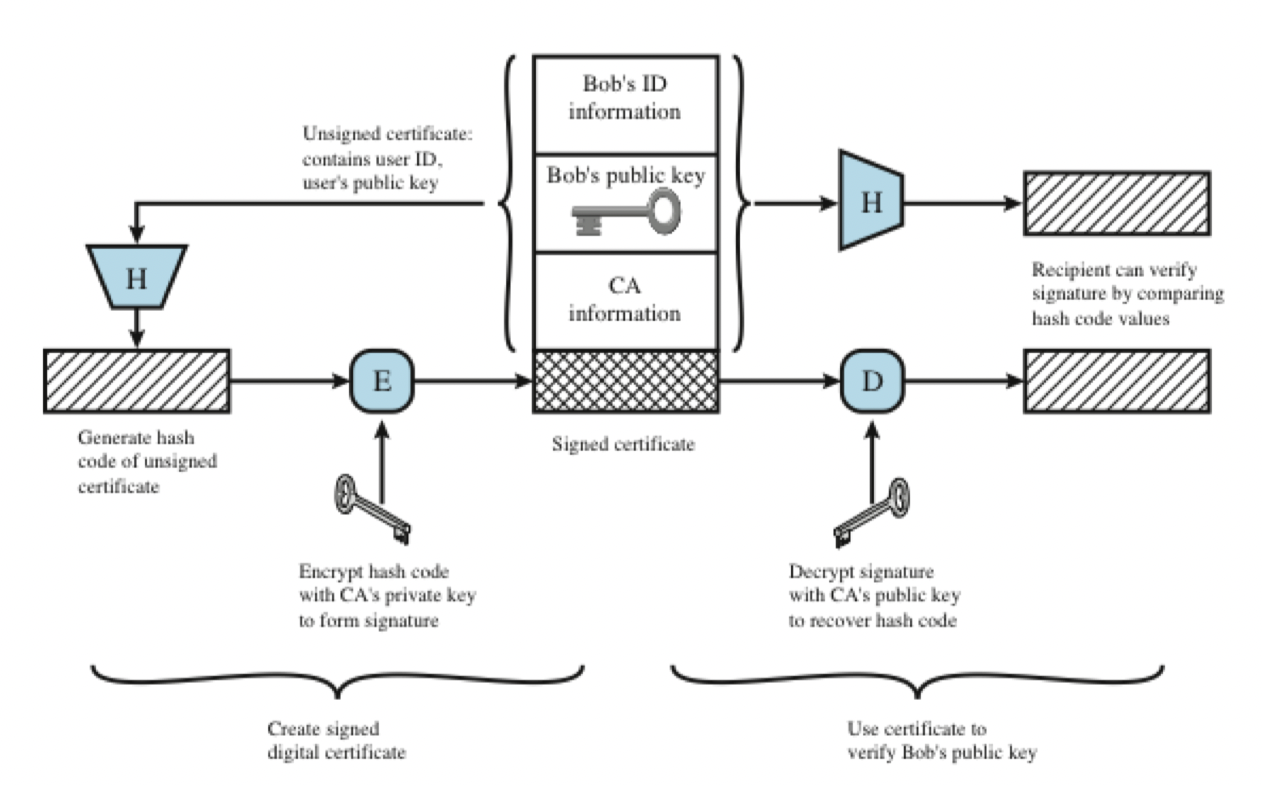
\includegraphics[scale=0.5]{images/certificate.png}}
\end{center}
The most common certificate format is \textbf{X.509}, containing a lot of information among which: serial number, issuer \& subject name, period of validity, signature.

\subsection{Certificate Lifecycle Management}
Lifecycle steps: enrollement, renewal \& revocation.
\subsubsection{Enrollement}
Enrollment is the process of obtaining a certificate from a CA.
\begin{enumerate}
    \item Alice generates a key pair, creates a message containing a copy of the public key and her identifying information, and signs the message with the private key (PKCS\#10).
    \begin{description}
    \item[Note:]Signing the message provided “proof-of-possession” (POP) of the private key as well as message integrity
    \end{description}
    \item CA verifies Alice’s signature on the message
    \item (Optional) CA verifies Alice’s ID through out-of-band means.
    \item CA creates a certificate containing the ID and public key, and signs it with the CA’s own key
    \begin{description}
    \item[Note:]CA has certified the binding between key and ID
    \end{description}
    \item Alice verifies the key, ID \& CA signature
    \item Alice and/or the CA publish the certificate
\end{enumerate}
\subsubsection{Revocation}
Each certificate includes a period of validity, but it may be desirable on occasion to revoke a certificate before it expires, for one of the following reasons:
\begin{itemize}
    \item The user’s private key is assumed to be compromised
    \item The user is no longer certified by this CA
    \item The CA’s certificate is assumed to be compromised
\end{itemize}
Each CA must maintain a \textit{Certification Revocation List} (CRL) consisting of all revoked but not expired certificates issued by that CA. Relying parties are expected to check CRLs before they rely on a certificate. Nevertheless, that are several problems with CRLs:
\begin{itemize}
    \item Not issued frequently enough to be effective against a serious attack
    \item Expensive to distribute (size \& bandwidth)
    \item Vulnerable to simple DOS attacks
    \item Can contain retroactive invalidity dates
    \item You can't revoke a CRL
\end{itemize}
For this reason, we use the \textit{Online Certs Status Protocol} (OCSP), that is designed for real-time responses to queries about the status of a single certificate (like a "selective" CRL).